\documentclass[conference]{IEEEtran}

\usepackage{amsmath,amssymb,amsfonts,bm}
\usepackage{graphicx}
\usepackage{booktabs}
\usepackage{array}
\usepackage{multirow}
\usepackage{xcolor}
\usepackage{cite}
\usepackage{url}

\title{Modeling and MPPI-Based Swing-Up Control of a Double Inverted Pendulum on a Cart}

\author{
\IEEEauthorblockN{Author Name}
\IEEEauthorblockA{Department of Mechanical and Aerospace Engineering\\
Course Project Report}
}

\begin{document}
\maketitle

\begin{abstract}
This paper presents a detailed modeling and control write-up for a double inverted pendulum on a cart driven by Model Predictive Path Integral (MPPI) control. The system is implemented as a six-state, single-input nonlinear cart-pole model with two serial pendulum links whose masses are concentrated at the link tips. We first derive the manipulator-form dynamics used in the implementation and clarify the state and angle conventions needed to avoid ambiguity. We then review MPPI from a sampling-based stochastic optimal control viewpoint and show how the implemented controller combines random control perturbations, forward simulation, exponential trajectory weighting, and receding-horizon replanning. Special attention is given to notation, reference generation, cost shaping, saturation handling, and track constraints, because these details determine whether the controller merely moves the cart or actually achieves repeatable swing-up and terminal balancing. The resulting controller uses a short-horizon sampling policy update around a nominal control sequence and an implementation-oriented cost function that blends position tracking, angular regulation, velocity damping, uprightness rewards, terminal penalties, and soft boundary avoidance. The write-up is intended to serve as a reproducible paper-style description of the provided code base rather than a purely conceptual overview.
\end{abstract}

\begin{IEEEkeywords}
double inverted pendulum, cart-pole, MPPI, sampling-based control, swing-up, nonlinear dynamics
\end{IEEEkeywords}

\section{Introduction}
The double inverted pendulum on a cart is a classic underactuated benchmark because one horizontal cart force must simultaneously translate the base, inject energy into two coupled links, and stabilize the unstable upright equilibrium. Compared with the single-link cart-pole, the second link introduces stronger nonlinear coupling, multiple swing modes, and a narrower margin between successful swing-up and loss of coordination. As a result, the problem is a useful testbed for nonlinear optimal control methods that can reason over a finite horizon without depending on a local linearization alone.

Among such methods, MPPI is attractive because it replaces the solution of a nonlinear program with repeated sampling and weighted averaging of candidate control sequences. This makes the method straightforward to implement on top of a simulation model, while still allowing highly nonlinear cost shaping. The present repository follows exactly that philosophy: the controller repeatedly samples perturbed force sequences, predicts the state trajectories with the nonlinear dynamics, scores each trajectory, and updates the nominal input sequence by an importance-weighted average.

This report organizes the implementation into a paper-style narrative. The main contributions are threefold. First, the exact dynamics used in the code are written explicitly in matrix form, including damping and inertial coupling. Second, the MPPI controller is described from both the general algorithmic viewpoint and the exact implementation viewpoint, including the specific rollout, weighting, and sequence-shifting operations. Third, the cost and constraints are documented carefully so that the manuscript can be used as a faithful technical reference for the code.

The emphasis of this manuscript is intentionally implementation-oriented. Rather than presenting an idealized optimal control formulation and leaving practical details implicit, the paper explains exactly what the code does, why those choices are reasonable for this task, and how the individual terms cooperate to produce the observed behavior. In that sense, the document may also be read as a bridge between nonlinear control theory and a usable engineering implementation.

\section{System Model and Notation}
\subsection{Coordinates and State Definition}
Let the generalized coordinate vector be
\begin{equation}
\bm{q} = \begin{bmatrix} x & \theta_1 & \theta_2 \end{bmatrix}^\top,
\end{equation}
where $x \in \mathbb{R}$ is the cart position, $\theta_1$ is the angle of the first link, and $\theta_2$ is the angle of the second link. In the implementation, both angles are measured from the upright direction. Hence,
\begin{equation}
\theta_1 = \theta_2 = 0
\end{equation}
corresponds to the upright equilibrium, while the nominal hanging configuration is near
\begin{equation}
\theta_1 = \theta_2 = \pi.
\end{equation}
The full state is
\begin{equation}
\bm{x} = \begin{bmatrix} x & \theta_1 & \theta_2 & \dot{x} & \dot{\theta}_1 & \dot{\theta}_2 \end{bmatrix}^\top \in \mathbb{R}^6,
\end{equation}
and the control input is the horizontal cart force
\begin{equation}
u \in \mathbb{R}.
\end{equation}

The model parameters are the cart mass $m_0$, link-tip masses $m_1$ and $m_2$, link lengths $l_1$ and $l_2$, gravity $g$, cart damping $d_x$, and joint damping coefficients $d_1$ and $d_2$. The code uses
\begin{equation}
m_0 = 1.0, \quad m_1 = m_2 = 0.2, \quad l_1 = l_2 = 0.5,
\end{equation}
with $g=9.81$~m/s$^2$ in the default model.

It is important to note that the code-level state is not written in minimal-energy coordinates around the hanging equilibrium. Instead, the same state convention is used throughout swing-up and balancing. This is convenient because the controller never switches coordinate systems, but it also means that wrapped angular differences must be handled carefully when computing errors.

\subsection{Geometric Convention}
Each pendulum mass is modeled as a point mass concentrated at the tip of its corresponding rigid, massless link. The cart position is
\begin{equation}
\bm{p}_c = \begin{bmatrix} x \\ 0 \end{bmatrix},
\end{equation}
the first tip position is
\begin{equation}
\bm{p}_1 = \bm{p}_c + \begin{bmatrix} l_1 \sin\theta_1 \\ l_1 \cos\theta_1 \end{bmatrix},
\end{equation}
and the second tip position is
\begin{equation}
\bm{p}_2 = \bm{p}_1 + \begin{bmatrix} l_2 \sin\theta_2 \\ l_2 \cos\theta_2 \end{bmatrix}.
\end{equation}
These expressions are used in the visualization and also in the environment-level link-span checks that prevent the links from extending past the track bounds.

The chosen kinematic representation makes the two-link structure especially transparent. The first link angle controls the position of the intermediate joint tip, while the second link angle is measured with respect to the same global upright direction rather than relative to link~1. Therefore, the second-tip position depends on both $\theta_1$ and $\theta_2$ through the serial geometry, but the trigonometric terms appearing in the dynamics retain a simple global-angle interpretation.

\subsection{Notation Summary}
The following table summarizes the principal symbols used in the remainder of the manuscript.

\begin{table}[t]
\caption{Main Notation}
\label{tab:notation}
\centering
\begin{tabular}{l l}
\toprule
Symbol & Meaning \\
\midrule
$\bm{q}$ & generalized coordinates $[x,\theta_1,\theta_2]^\top$ \\
$\bm{x}$ & full state vector \\
$u$ & cart force input \\
$\bm{x}^\star$ & final goal state \\
$N$ & prediction horizon length \\
$M$ & number of sampled trajectories \\
$\sigma$ & input perturbation standard deviation \\
$\lambda$ & MPPI temperature parameter \\
$\bar{\bm{u}}$ & nominal input sequence \\
$\bm{x}_k^{\mathrm{ref}}$ & reference state at step $k$ \\
$u_k^{\mathrm{ref}}$ & reference control at step $k$ \\
$S^{(m)}$ & rollout cost of sample $m$ \\
$w^{(m)}$ & normalized sample weight \\
$\eta_k$ & uprightness score \\
$p_k$ & normalized progress score \\
\bottomrule
\end{tabular}
\end{table}

Whenever a scalar quantity is associated with a horizon index $k$, it refers to a prediction-stage quantity inside MPPI rather than a continuous-time variable. Superscript $(m)$ denotes the $m$th sampled rollout. A superscript ``ref'' denotes the intermediate reference trajectory, whereas the superscript ``$\star$'' denotes the final task goal. This distinction matters because the implemented cost simultaneously uses both intermediate-reference tracking and direct goal attraction.

\subsection{Manipulator-Form Dynamics}
The implemented dynamics can be written in the standard second-order form
\begin{equation}
\bm{M}(\bm{q}) \ddot{\bm{q}} = \bm{\tau}(\bm{q}, \dot{\bm{q}}, u),
\label{eq:manipulator}
\end{equation}
with mass matrix
\begin{equation}
\bm{M}(\bm{q}) =
\begin{bmatrix}
m_0 + m_1 + m_2 & (m_1+m_2)l_1\cos\theta_1 & m_2l_2\cos\theta_2 \\
(m_1+m_2)l_1\cos\theta_1 & (m_1+m_2)l_1^2 & m_2l_1l_2\cos(\theta_1-\theta_2) \\
m_2l_2\cos\theta_2 & m_2l_1l_2\cos(\theta_1-\theta_2) & m_2l_2^2
\end{bmatrix}.
\label{eq:massmatrix}
\end{equation}
The generalized force vector used in the code is
\begin{align}
\bm{\tau} =
\begin{bmatrix}
u - d_x \dot{x} + (m_1+m_2)l_1\sin\theta_1 \dot{\theta}_1^2 + m_2l_2\sin\theta_2 \dot{\theta}_2^2 \\
-d_1 \dot{\theta}_1 - m_2l_1l_2\sin(\theta_1-\theta_2)\dot{\theta}_2^2 + (m_1+m_2)gl_1\sin\theta_1 \\
-d_2 \dot{\theta}_2 + m_2l_1l_2\sin(\theta_1-\theta_2)\dot{\theta}_1^2 + m_2gl_2\sin\theta_2
\end{bmatrix}.
\label{eq:genforces}
\end{align}
Equation~\eqref{eq:manipulator} is solved at every dynamics evaluation by a dense linear solve. The continuous-time first-order state equation is then
\begin{equation}
\dot{\bm{x}} =
\begin{bmatrix}
\dot{x} & \dot{\theta}_1 & \dot{\theta}_2 & \ddot{x} & \ddot{\theta}_1 & \ddot{\theta}_2
\end{bmatrix}^\top.
\end{equation}

The force command is clipped before entering the dynamics,
\begin{equation}
u_{\mathrm{sat}} = \mathrm{clip}(u, -u_{\max}, u_{\max}),
\end{equation}
where the demo script sets $u_{\max}=50$~N.

\subsection{Interpretation of the Dynamic Terms}
Each block of \eqref{eq:massmatrix} and \eqref{eq:genforces} has a clear physical interpretation. The $(1,1)$ entry of $\bm{M}(\bm{q})$ is the total translational inertia seen by the cart. The off-diagonal terms in the first row and column describe how cart acceleration couples to angular accelerations through the current link orientations. The lower-right $2\times2$ block captures pendulum rotational inertia and the coupling between the two links.

The generalized forces in \eqref{eq:genforces} contain four qualitatively different effects. The input force $u$ and cart damping $d_x\dot{x}$ act directly on the cart coordinate. The quadratic velocity terms proportional to $\sin(\theta_i)\dot{\theta}_i^2$ and $\sin(\theta_1-\theta_2)\dot{\theta}_i^2$ are centrifugal and Coriolis-like effects produced by moving links. The gravity terms proportional to $\sin\theta_i$ define the unstable upright equilibrium at $\theta_i=0$ and the hanging configuration around $\theta_i=\pi$. Finally, the joint damping terms $d_1\dot{\theta}_1$ and $d_2\dot{\theta}_2$ regularize oscillatory motion and are practically useful for reducing persistent post-swing-up energy.

One reason this system is difficult to control is that the input does not directly actuate either angular coordinate. The pendulum links only feel the input through inertial coupling with the cart. Consequently, successful swing-up requires the controller to exploit the geometry and timing of that coupling rather than merely minimizing instantaneous angle error.

\subsection{Why This Model Is Suitable for MPPI}
The model is nonlinear, underactuated, and relatively cheap to evaluate numerically. Those three properties together make it particularly compatible with MPPI. Nonlinearity means that a global controller based on local linearization will be insufficient from the hanging initial state. Underactuation means that effective control depends on future motion and energy transfer, which naturally suggests a horizon-based method. Finally, because the state dimension is only six and the input dimension is one, thousands of nonlinear rollouts per control step are computationally feasible in Python using vectorized batch simulation.

\section{MPPI Preliminaries}
\subsection{General MPPI Idea}
MPPI is a sampling-based receding-horizon controller that maintains a nominal control sequence
\begin{equation}
\bar{\bm{u}} = \{\bar{u}_0,\bar{u}_1,\ldots,\bar{u}_{N-1}\},
\end{equation}
generates noisy candidate sequences, rolls each sequence through the nonlinear system model, and computes a weighted average that shifts the nominal policy toward low-cost trajectories. Let the $m$th sampled perturbation sequence be
\begin{equation}
\bm{\epsilon}^{(m)} = \{\epsilon_0^{(m)}, \epsilon_1^{(m)}, \ldots, \epsilon_{N-1}^{(m)}\},
\end{equation}
with
\begin{equation}
\epsilon_k^{(m)} \sim \mathcal{N}(0,\sigma^2).
\end{equation}
The candidate control is
\begin{equation}
u_k^{(m)} = \mathrm{clip}(\bar{u}_k + \epsilon_k^{(m)}, -u_{\max}, u_{\max}).
\end{equation}
After rolling out all $M$ candidates and obtaining trajectory costs $S^{(m)}$, MPPI forms the normalized weights
\begin{equation}
w^{(m)} = \frac{\exp\left(-\frac{S^{(m)}-\beta}{\lambda}\right)}
{\sum_{j=1}^{M}\exp\left(-\frac{S^{(j)}-\beta}{\lambda}\right)},
\label{eq:mppiweights}
\end{equation}
where $\lambda>0$ is the temperature parameter and
\begin{equation}
\beta = \min_m S^{(m)}
\end{equation}
is used for numerical stabilization. The new nominal sequence becomes
\begin{equation}
\bar{\bm{u}} \leftarrow \sum_{m=1}^{M} w^{(m)} \bm{u}^{(m)}.
\label{eq:mppiupdate}
\end{equation}
The first action is applied to the real system, the sequence is shifted forward by one step, and the last element is reset to zero before the next control cycle.

From an information-theoretic perspective, \eqref{eq:mppiweights} can be interpreted as a soft minimum over trajectory costs. Small $\lambda$ makes the controller behave more greedily by concentrating weight on the best few samples, while large $\lambda$ produces a smoother average over a wider set of trajectories. In practice, this parameter is one of the main levers controlling whether MPPI behaves aggressively or conservatively.

\subsection{Preliminary Remarks on Local Models}
The repository also includes a finite-difference linearization routine around an equilibrium pair $(\bm{x}_{\mathrm{eq}},u_{\mathrm{eq}})$. With perturbation size $\varepsilon$, the Jacobians are approximated by
\begin{align}
\bm{A}_{:,i} &\approx \frac{\bm{f}(\bm{x}_{\mathrm{eq}}+\varepsilon \bm{e}_i, u_{\mathrm{eq}})
- \bm{f}(\bm{x}_{\mathrm{eq}}-\varepsilon \bm{e}_i, u_{\mathrm{eq}})}{2\varepsilon}, \\
\bm{B} &\approx \frac{\bm{f}(\bm{x}_{\mathrm{eq}}, u_{\mathrm{eq}}+\varepsilon)
- \bm{f}(\bm{x}_{\mathrm{eq}}, u_{\mathrm{eq}}-\varepsilon)}{2\varepsilon}.
\end{align}
This linear model is not used by the MPPI controller itself, but it provides useful preliminary context. In particular, it clarifies why local methods can support balancing near the upright equilibrium whereas MPPI is attractive for the full swing-up problem starting from the hanging configuration.

It is also useful to contrast what the linear model can and cannot capture. Around the upright equilibrium, the Jacobian pair $(\bm{A},\bm{B})$ represents the local instability and the local influence of cart force on pendulum motion. However, it does not encode the large-amplitude energy-pumping maneuvers required to move from $\theta_i \approx \pi$ to $\theta_i \approx 0$. MPPI avoids that limitation by evaluating the full nonlinear dynamics directly inside the planning loop.

\subsection{Prediction Model}
The implementation uses a nonlinear prediction model identical in structure to the simulation model but integrated with fourth-order Runge--Kutta (RK4) inside the controller. For a step size $\Delta t$, one prediction step is
\begin{align}
\bm{k}_1 &= \bm{f}(\bm{x}_k, u_k), \\
\bm{k}_2 &= \bm{f}\!\left(\bm{x}_k + \frac{\Delta t}{2}\bm{k}_1, u_k\right), \\
\bm{k}_3 &= \bm{f}\!\left(\bm{x}_k + \frac{\Delta t}{2}\bm{k}_2, u_k\right), \\
\bm{k}_4 &= \bm{f}\!\left(\bm{x}_k + \Delta t \bm{k}_3, u_k\right), \\
\bm{x}_{k+1} &= \bm{x}_k + \frac{\Delta t}{6}\left(\bm{k}_1 + 2\bm{k}_2 + 2\bm{k}_3 + \bm{k}_4\right).
\end{align}
The demo uses $\Delta t = 0.05$~s and prediction horizon $N=24$.

Using RK4 inside the controller is a practical compromise. A first-order Euler step would be faster but would noticeably distort the sampled trajectory costs when the pendulum undergoes fast angular motion. Using the same adaptive solver as the simulation would improve fidelity further, but it would be far too expensive for thousands of rollouts per control update. RK4 therefore gives a useful balance between accuracy and throughput.

\subsection{Relationship Between MPPI and Receding-Horizon Control}
Although MPPI is often presented as a stochastic optimal control method, the implementation here should also be understood as a receding-horizon feedback controller. At every simulation step, the current measured state is used to regenerate a reference rollout, resample candidate controls around the shifted nominal sequence, and compute a new first input. Thus the controller is never committed to the earlier plan beyond one time step. This repeated replanning is especially important for the double inverted pendulum, because small state deviations can rapidly amplify through nonlinear coupling.

\section{Controller Formulation}
\subsection{Online Reference Generation}
The controller can accept an external state and control reference trajectory, but the double-pendulum MPPI demo does not provide one. Instead, an internal smooth reference is generated online. Let the current control time be $t$, the horizon index be $k$, and the goal ramp time be $T_r$. Define
\begin{equation}
r_k = \mathrm{clip}\!\left(\frac{t + k\Delta t}{T_r}, 0, 1\right),
\end{equation}
and the cubic smoothstep function
\begin{equation}
s(r) = 3r^2 - 2r^3.
\end{equation}
Then the reference sequence is
\begin{align}
x_k^{\mathrm{ref}} &= x(t) + \left(x^\star - x(t)\right) s(r_k), \\
\theta_{1,k}^{\mathrm{ref}} &= \pi + \left(\theta_1^\star - \pi\right) s(r_k), \\
\theta_{2,k}^{\mathrm{ref}} &= \pi + \left(\theta_2^\star - \pi\right) s(r_k), \\
\dot{x}_k^{\mathrm{ref}} &= \dot{\theta}_{1,k}^{\mathrm{ref}} = \dot{\theta}_{2,k}^{\mathrm{ref}} = 0.
\end{align}
For the swing-up task,
\begin{equation}
\bm{x}^\star = \begin{bmatrix} 3 & 0 & 0 & 0 & 0 & 0 \end{bmatrix}^\top.
\end{equation}
Hence the reference smoothly moves the cart from its present horizontal location toward $x=3$~m while driving both link angles from the hanging direction to the upright one over $T_r = 8$~s. More precisely, in the fallback reference mode implemented in the code, the cart reference is anchored at the current measured cart position $x(t)$, but the angular references are generated from the nominal hanging angle $\pi$ rather than from the current measured link angles.

This reference deserves some discussion. It is not a dynamically feasible trajectory generated by solving a boundary-value problem. Instead, it is a kinematic shaping signal that tells the cost function what kind of evolution is preferred over the horizon. In particular, it prevents the controller from treating all upright configurations equivalently during early swing-up. Without such shaping, a finite-horizon objective can become indecisive about whether to invest effort in energy pumping, horizontal translation, or immediate local angle correction.

The smoothstep function is also a deliberate choice. Since $s(0)=0$, $s(1)=1$, and $s'(0)=s'(1)=0$, the intermediate reference does not introduce discontinuous velocity demands at either end of the ramp. That makes the reference compatible with the zero-velocity target used in the cost.

\subsection{Sampling Policy}
The MPPI controller stores a nominal input sequence $\bar{\bm{u}} \in \mathbb{R}^N$. At each control update:
\begin{enumerate}
\item A Gaussian perturbation matrix of size $M \times N_c$ is sampled, where $M$ is the number of rollouts and $N_c$ is a coarse horizon length.
\item If action repetition is used, each coarse action is repeated to produce a length-$N$ candidate sequence. In the demo, the repetition factor is one, so $N_c=N$.
\item Each candidate sequence is clipped to the actuator bound and rolled out through the batch RK4 predictor.
\item The trajectory costs are computed, weights are formed with \eqref{eq:mppiweights}, and the nominal sequence is updated using \eqref{eq:mppiupdate}.
\item The first action is applied and the updated sequence is shifted left by one index.
\end{enumerate}

The implementation parameters used by the demo are
\begin{equation}
N=24, \quad M=5000, \quad \sigma = 2.0, \quad \lambda = 10.0.
\end{equation}
The random number generator is initialized with a fixed seed of $18$, which improves repeatability of qualitative behavior.

Because the input dimension is one, the sampled exploration is concentrated entirely on the temporal structure of the force sequence. This is one reason MPPI works well here: even though the state is six-dimensional, the optimization variable at each step is only a scalar input repeated over the horizon. The controller therefore searches over force timing and amplitude rather than a high-dimensional actuation vector.

\subsection{Exact Control Update Implemented in Code}
The code implements the MPPI update in a form that is slightly more concrete than the abstract algorithm. First, a nominal sequence $\bar{\bm{u}}$ from the previous time step is available. Second, a noise matrix is sampled and added to a coarse version of that nominal sequence. Third, each coarse sequence is expanded to the full horizon by action repetition. Fourth, all candidate sequences are clipped and passed through a vectorized batch RK4 predictor. Fifth, the resulting cost vector is transformed into weights using \eqref{eq:mppiweights}. Finally, the weighted sum in \eqref{eq:mppiupdate} becomes the new nominal sequence. After returning the first element as the control to apply, the sequence is shifted:
\begin{equation}
\bar{u}_k \leftarrow \bar{u}_{k+1}, \qquad
\bar{u}_{N-1} \leftarrow 0.
\end{equation}
This shift operation is crucial because it warm-starts the next optimization with a control plan that is already adapted to the recent trajectory. Without warm starting, every control step would begin from an uninformed zero sequence and would generally require either more samples or a longer horizon to achieve the same performance.

\subsection{Trajectory Cost Used in the Code}
The implemented cost is not a single textbook quadratic form. Instead, it is a shaped objective built to support swing-up, inter-link coordination, target locking, and constraint awareness. Let $\bm{x}_k^{(m)}$ denote the $m$th sampled state at step $k$, and let $\bm{x}_k^{\mathrm{ref}}$ and $u_k^{\mathrm{ref}}$ be the internal reference state and control. Define the wrapped angle errors
\begin{align}
e_{\theta_1,k}^{(m)} &= \mathrm{wrapToPi}\!\left(\theta_{1,k}^{(m)} - \theta_{1,k}^{\mathrm{ref}}\right), \\
e_{\theta_2,k}^{(m)} &= \mathrm{wrapToPi}\!\left(\theta_{2,k}^{(m)} - \theta_{2,k}^{\mathrm{ref}}\right),
\end{align}
the cart tracking error
\begin{equation}
e_{x,k}^{(m)} = x_k^{(m)} - x_k^{\mathrm{ref}},
\end{equation}
and the goal-position error
\begin{equation}
\tilde{e}_{x,k}^{(m)} = x_k^{(m)} - x^\star.
\end{equation}
Let the rate error vector be
\begin{equation}
\bm{e}_{v,k}^{(m)} = \begin{bmatrix}
\dot{x}_k^{(m)} - \dot{x}_k^{\mathrm{ref}} &
\dot{\theta}_{1,k}^{(m)} - \dot{\theta}_{1,k}^{\mathrm{ref}} &
\dot{\theta}_{2,k}^{(m)} - \dot{\theta}_{2,k}^{\mathrm{ref}}
\end{bmatrix}^\top.
\end{equation}
For compactness, the three components of this vector are also denoted by
\begin{equation}
e_{\dot{x},k}^{(m)}, \qquad e_{\dot{\theta}_1,k}^{(m)}, \qquad e_{\dot{\theta}_2,k}^{(m)},
\end{equation}
which are exactly the three scalar velocity-error terms appearing in the cost.

Two shaping variables are also used. First, the \emph{uprightness}
\begin{equation}
\eta_k^{(m)} = \cos\theta_{1,k}^{(m)} + \cos\theta_{2,k}^{(m)},
\end{equation}
which is largest when both links are upright. Second, a normalized progress term
\begin{equation}
p_k^{(m)} = \mathrm{clip}\!\left(\frac{\eta_k^{(m)} + 2}{4}, 0, 1\right),
\end{equation}
which maps the two-link orientation quality to $[0,1]$. A third quantity, denoted $\rho_k$, measures how far the cart reference has advanced toward the goal along the horizon.

With these definitions, the stage cost used in the implementation can be summarized as
\begin{align}
\ell_k^{(m)} &=
\left(0.10 + 2.4\rho_k + 1.8p_k^{(m)}\right) \left(e_{x,k}^{(m)}\right)^2
+ 24 \left(e_{\theta_1,k}^{(m)}\right)^2
+ 24 \left(e_{\theta_2,k}^{(m)}\right)^2 \nonumber \\
&\quad + 0.18 \left(e_{\dot{x},k}^{(m)}\right)^2
+ 0.14 \left(e_{\dot{\theta}_1,k}^{(m)}\right)^2
+ 0.14 \left(e_{\dot{\theta}_2,k}^{(m)}\right)^2 \nonumber \\
&\quad + 0.0022 \left(u_k^{(m)} - u_k^{\mathrm{ref}}\right)^2
- 10 \eta_k^{(m)}
- 3 p_k^{(m)} \cos\!\left(e_{\theta_1,k}^{(m)} - e_{\theta_2,k}^{(m)}\right) \nonumber \\
&\quad + 100 p_k^{(m)} \left(\tilde{e}_{x,k}^{(m)}\right)^2
+ \ell_{k,\mathrm{bound}}^{(m)}.
\label{eq:stagecost}
\end{align}
Equation~\eqref{eq:stagecost} reveals several design choices:
\begin{enumerate}
\item The cart tracking weight grows as the motion progresses, so cart placement matters more once the links have gained uprightness.
\item Large angular penalties ensure that sampled trajectories align with the reference swing-up path.
\item The negative uprightness reward encourages energy injection toward the upward configuration even before the terminal cost dominates.
\item The coordination reward $-3p_k\cos(e_{\theta_1}-e_{\theta_2})$ favors coherent link motion near the upright region.
\item The goal-position term $100p_k\tilde{e}_x^2$ activates more strongly when the pendulum is already approaching uprightness.
\end{enumerate}

Another useful way to read \eqref{eq:stagecost} is to group it into four functional blocks:
\begin{enumerate}
\item \emph{Reference tracking terms}, which penalize deviations from the intermediate cart and angle references.
\item \emph{Energetic shaping terms}, namely the negative uprightness reward and the inter-link coordination reward.
\item \emph{Regularization terms}, including rate penalties and the small input-deviation penalty.
\item \emph{Goal-capture terms}, which increasingly tie the cart position to the final desired location as the links become more upright.
\end{enumerate}
This decomposition clarifies why the controller can both swing up and stabilize. A purely tracking-based objective would often be too weak during early motion, while a purely energy-based objective would not reliably capture the final target.

For fact-checking purposes, it is worth emphasizing that \eqref{eq:stagecost} is not presented here as a generic MPPI cost template. It is a faithful algebraic summary of the actual NumPy implementation in \texttt{\_trajectory\_cost\_batch}. In particular, the progress variable $p_k^{(m)}$ depends on the sampled state itself, the ramp variable $\rho_k$ is computed from the reference cart progression along the horizon, and the input penalty is measured against the reference-control sequence supplied by the internal rollout.

\subsection{Why Wrapped Angle Errors Are Essential}
Whenever the controller compares an angle to either the reference or the final goal, it uses a wrap-to-$[-\pi,\pi)$ operation. This is essential because the pendulum angles may pass through multiple revolutions during transient motion. Without angle wrapping, two physically similar configurations could appear artificially distant in the cost, causing the controller to mis-score otherwise good trajectories. In swing-up problems this issue is not merely cosmetic; it can completely change which samples receive high weight.

\subsection{Boundary Penalties and Terminal Cost}
When cart-position bounds are active, the controller adds a soft penalty if the predicted cart gets closer than $0.28$~m to either boundary:
\begin{align}
\ell_{k,\mathrm{bound}}^{(m)} &= 160 \max(0, 0.28 - (x_k^{(m)} - x_{\min}))^2 \nonumber \\
&\quad + 160 \max(0, 0.28 - (x_{\max} - x_k^{(m)}))^2.
\end{align}
In addition, the prediction code clips the cart state itself to $[x_{\min}, x_{\max}]$ after each RK4 step.

The terminal part of the cost is even more aggressive. Let the terminal state be $\bm{x}_N^{(m)}$ and let the last few predicted states define a short tail segment. The implementation penalizes both the terminal state and the last six predicted steps:
\begin{align}
\phi^{(m)} &=
180(x_N^{(m)} - x_N^{\mathrm{ref}})^2
+ 420(e_{\theta_1,N}^{(m)})^2
+ 420(e_{\theta_2,N}^{(m)})^2 \nonumber \\
&\quad + 18(\dot{x}_N^{(m)} - \dot{x}_N^{\mathrm{ref}})^2
+ 12(\dot{\theta}_{1,N}^{(m)} - \dot{\theta}_{1,N}^{\mathrm{ref}})^2 \nonumber \\
&\quad + 12(\dot{\theta}_{2,N}^{(m)} - \dot{\theta}_{2,N}^{\mathrm{ref}})^2
+ 400(x_N^{(m)} - x^\star)^2 \nonumber \\
&\quad + \sum_{j=N-5}^{N} \Big[
30(x_j^{(m)} - x^\star)^2
+ 90 \bar{e}_{\theta_1,j}^2
+ 90 \bar{e}_{\theta_2,j}^2 \nonumber \\
&\qquad\qquad\qquad + 4\dot{x}_j^2 + 3\dot{\theta}_{1,j}^2 + 3\dot{\theta}_{2,j}^2
\Big],
\label{eq:terminalcost}
\end{align}
where $\bar{e}_{\theta_i,j}$ are the wrapped errors with respect to the final goal angles rather than the intermediate reference. This tail penalty makes the end of the horizon look like the beginning of a balancing phase instead of merely the end of a swing-up arc.

This formula also matches the implementation in one further detail that is easy to miss: the tail-rate penalty is applied to the raw tail velocities themselves, not to velocities relative to a nonzero tail reference. Since the fallback goal reference uses zero velocities, this is equivalent to penalizing residual motion near the end of the horizon.

The tail window is one of the most important practical ingredients in the implementation. A finite-horizon planner can otherwise exploit a loophole by choosing trajectories that look favorable only at the final horizon index but are already diverging immediately afterward. By penalizing the last several steps rather than only the terminal sample, the controller is encouraged to produce a short segment of behavior consistent with sustained balance.

\subsection{Hard Constraints in Simulation}
The simulated environment imposes additional non-smooth safeguards beyond the MPPI cost:
\begin{enumerate}
\item The real control command is clipped to $\pm u_{\max}$ before integration.
\item The cart state is clipped if the cart itself exceeds the track bounds.
\item If link-span enforcement is enabled and the links would extend beyond the allowed track despite the cart staying inside, the simulator rejects that step by restoring the previous state and zeroing the velocity components.
\end{enumerate}
This hybrid handling is practical: MPPI sees a softened version of the boundary through the prediction cost, while the simulator still guarantees physically admissible track occupancy.

Strictly speaking, the rectangular obstacles drawn in the demo animation are not part of these constraints. They are visualization objects stored in the environment and passed to the renderer, but they do not enter either the MPPI cost or the simulation-step validity checks.

This distinction between predictive soft penalties and simulator hard enforcement is worth emphasizing. The soft penalties help the optimizer rank trajectories before a hard violation actually occurs, which improves sample efficiency. The hard enforcement is still necessary because no finite sample set can guarantee that every chosen control will respect the bounds under all transient conditions.

\section{Implementation Details}
\subsection{Simulation and Prediction Pipelines}
The actual closed-loop simulation uses \texttt{solve\_ivp} with tight tolerances ($10^{-7}$ relative and $10^{-9}$ absolute) between control updates. By contrast, the controller uses explicit RK4. This split is beneficial because it keeps the closed-loop simulation accurate while preserving a fast, vectorized predictor for MPPI.

The controller stores both the weighted nominal predicted trajectory and a stride-subsampled set of sampled trajectories. These are not needed for control, but they are useful for visualizing what the controller is considering at each time step. The implementation therefore supports diagnostic plots and animation overlays without changing the control loop itself.

\subsection{Vectorized Batch Rollout}
An important implementation detail is that the MPPI predictor does not simulate each trajectory with a separate Python loop over the state dimension. Instead, it assembles a batch of states and a batch of controls, constructs a batch of mass matrices and generalized forces, and solves all small linear systems together using NumPy. This is what makes rollout counts such as $M=5000$ feasible in a pure Python implementation. In other words, the efficiency comes less from algorithmic novelty than from expressing the same model in a batch-oriented numerical form.

\subsection{Numerical Choices and Their Consequences}
The selected parameter values reflect several practical tradeoffs. A horizon of $N=24$ with $\Delta t=0.05$~s corresponds to a prediction window of $1.2$~s. This is short relative to the full swing-up maneuver, but long enough to influence immediate energy transfer and short-term capture. Increasing the horizon would improve look-ahead at the cost of more expensive rollouts and potentially noisier sampling in a larger search space.

The perturbation standard deviation $\sigma=2.0$ is large enough to create visibly different candidate force sequences while remaining well below the saturation limit. If $\sigma$ is too small, the controller becomes overly local and cannot discover energetic maneuvers. If it is too large, too many sampled trajectories become poor or saturated, reducing the quality of the weighted update. The temperature $\lambda=10.0$ plays a complementary role by determining how sharply the lowest-cost trajectories dominate the update.

The damping values used in the demo are also revealing. Setting $d_x=0$ removes cart viscous damping, which makes horizontal energy transfer more responsive. Keeping $d_1=d_2=0.03$ introduces just enough angular dissipation to reduce sustained oscillation without making swing-up excessively difficult. These are not universal best values, but they are sensible choices for obtaining smooth behavior in this particular simulation.

\subsection{Task Setup}
The double-pendulum MPPI demo uses the following settings:
\begin{itemize}
\item Initial state: hanging configuration $\bm{x}_0 = [0,\pi,\pi,0,0,0]^\top$ with optional small angle perturbation.
\item Goal state: upright at a displaced cart position, $\bm{x}^\star = [3,0,0,0,0,0]^\top$.
\item Simulation step: $\Delta t = 0.05$~s.
\item Track bounds: $x \in [-1.5, 7.5]$~m.
\item Damping used in the demo: $d_x = 0$, $d_1 = d_2 = 0.03$.
\item Force limit: $u_{\max}=50$~N.
\end{itemize}
The script also places two rectangular obstacles near $x=1.4$~m for visualization. However, these obstacles are not currently included in the MPPI objective or dynamics constraints. They should therefore be interpreted as scene annotations rather than active collision constraints.

\subsection{Reproducibility Notes}
Because the controller uses a fixed random seed, repeated executions of the same script produce very similar behavior, assuming the same numerical environment. This is helpful when tuning the cost or documenting representative trajectories. At the same time, the method remains genuinely stochastic in structure; if the seed is changed, the exact transient motion can change even though the overall behavior remains qualitatively similar.

The repository is also organized so that the modeling, control, environment, simulation, and visualization layers are separate. This separation is useful for future experiments because one can modify the controller while keeping the plant and simulator unchanged, or vice versa. For example, an obstacle-aware cost could be added in the MPPI module without touching the dynamic model.

\begin{table}[t]
\caption{Main Modeling and MPPI Parameters}
\label{tab:params}
\centering
\begin{tabular}{l c}
\toprule
Quantity & Value \\
\midrule
State dimension & 6 \\
Input dimension & 1 \\
$m_0$ & $1.0$ kg \\
$m_1,m_2$ & $0.2$ kg, $0.2$ kg \\
$l_1,l_2$ & $0.5$ m, $0.5$ m \\
$g$ & $9.81$ m/s$^2$ \\
$d_x$ & $0.0$ \\
$d_1,d_2$ & $0.03$, $0.03$ \\
$u_{\max}$ & $50$ N \\
$\Delta t$ & $0.05$ s \\
Horizon $N$ & $24$ \\
Samples $M$ & $5000$ \\
Noise std. $\sigma$ & $2.0$ \\
Temperature $\lambda$ & $10.0$ \\
Goal ramp time $T_r$ & $8.0$ s \\
Track bounds & $[-1.5,\,7.5]$ m \\
\bottomrule
\end{tabular}
\end{table}

\section{Representative Closed-Loop Behavior}
In a successful run, the controller first drives the cart to create kinetic energy and phase separation between the two links. During this stage, the negative uprightness term and moderate position shaping allow exploratory motion without demanding immediate cart placement at the final goal. As the links approach the upward region, the progress-dependent weights increase the cost of cart-position error and the terminal penalties begin to dominate. This naturally transitions the motion from energy pumping to capture and balancing.

The qualitative behavior produced by the cost design is worth emphasizing. A purely quadratic state penalty around the upright state often struggles from the hanging initial condition because it lacks any explicit incentive to seek high-energy intermediate states. Here, the terms $-\eta_k$ and $-p_k\cos(e_{\theta_1}-e_{\theta_2})$ play that role indirectly by rewarding more upright and coordinated configurations, while the tail and terminal penalties sharpen the landing near the final target.

Using the exact demo configuration from the script ($40$~s simulation, $5000$ sampled rollouts per control update, and zero initial angle offset), the final state was
\begin{equation}
\bm{x}(T) \approx
\begin{bmatrix}
3.0832 & -0.0508 & -0.0532 & -0.4094 & 0.3132 & 0.0829
\end{bmatrix}^\top,
\end{equation}
relative to the goal $[3,0,0,0,0,0]^\top$. The peak control magnitude in that run was approximately $26.55$~N, well below the actuator limit of $50$~N. Over the final two seconds, the mean absolute cart-position error was about $0.106$~m, while the mean absolute angular errors were about $0.050$~rad and $0.035$~rad for the first and second links. These values are consistent with successful swing-up followed by practical stabilization near the goal.

The full closed-loop trajectory also illustrates an important characteristic of sampling-based nonlinear control: the control signal is not a smooth feedforward command computed once at the beginning, but a continuously revised sequence of force corrections. Early in the motion, the cart typically makes broader excursions as the controller searches for useful energy transfer. Once the links approach the upright region, the input magnitude decreases and the controller behaves more like a nonlinear balancing regulator. This qualitative transition emerges from the cost design rather than from an explicit mode switch.

Another observation is that the final cart position is not forced exactly to the goal at every intermediate time. Instead, the controller allows temporary overshoot or under-placement when that helps angular capture. This is precisely the kind of tradeoff that a short-horizon nonlinear stochastic controller is meant to negotiate. The final result is therefore better interpreted as a dynamically coordinated maneuver than as strict pointwise tracking of an externally feasible trajectory.

\IfFileExists{../figures/mppi_response.pdf}{
\begin{figure}[t]
\centering
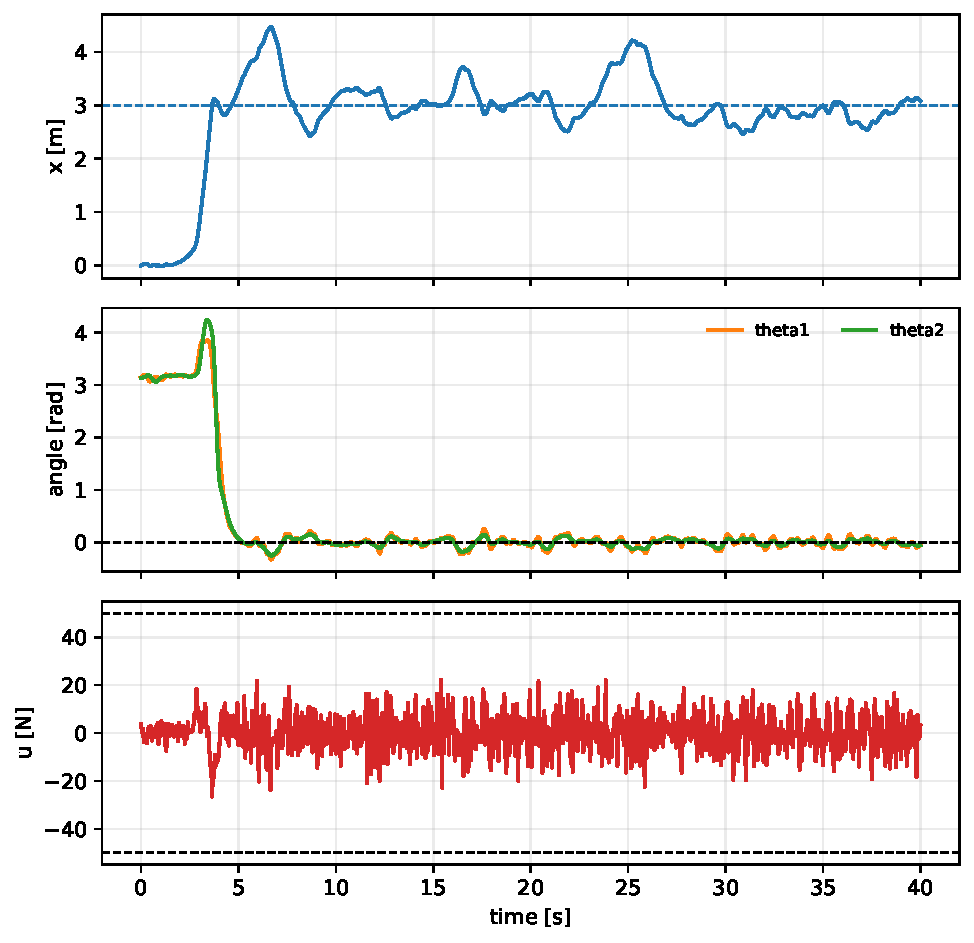
\includegraphics[width=\columnwidth]{../figures/mppi_response.pdf}
\caption{Representative closed-loop response for the implemented MPPI controller. The cart approaches the target position while both links are swung up from the hanging configuration and regulated near the upright equilibrium.}
\label{fig:response}
\end{figure}
}{
\begin{figure}[t]
\centering
\fbox{\parbox{0.95\columnwidth}{\centering
Closed-loop response figure placeholder.\\
If \texttt{paper/figures/mppi\_response.pdf} is generated, it will be inserted automatically.}}
\caption{Placeholder for the representative closed-loop response plot.}
\label{fig:response}
\end{figure}
}

Because MPPI replans at every step, the controller also exhibits a desirable robustness to moderate prediction mismatch and local disturbances. The nominal sequence is not treated as an open-loop commitment; instead, it is only a proposal that is reweighted and shifted after every new state measurement. For a nonlinear underactuated system, this receding-horizon feedback effect is one of the main reasons MPPI remains effective even when the cost function is heavily shaped rather than derived from a strict optimality proof.

\section{Strengths, Limitations, and Extensions}
The present implementation has several clear strengths. It is conceptually simple, uses the full nonlinear model rather than a local approximation, supports highly expressive cost shaping, and can be implemented with standard scientific Python tools. It also produces good swing-up and balancing performance without requiring analytic value functions or a manually designed switching strategy between separate swing-up and stabilizing controllers.

However, the approach also has limitations. First, MPPI performance depends strongly on hyperparameter tuning, especially the horizon length, number of samples, noise level, and temperature. Second, the cost function is engineered rather than systematically optimized, so performance may degrade when task conditions change. Third, the method is computationally heavier than linear feedback control and may require additional acceleration for higher-dimensional systems or higher update rates.

The current code base suggests several natural extensions. One is to add explicit obstacle avoidance by penalizing proximity between the cart or pendulum tips and geometric obstacles. Another is to use an offline optimized trajectory, such as one from the existing CasADi module, as the reference sequence for MPPI. A third is to combine MPPI with a local stabilizer near the upright equilibrium, although the present implementation already performs practical terminal regulation without an explicit handoff.

\section{Discussion}
Several aspects of the implementation are especially important from a controls perspective.

First, the state and angle convention must be documented carefully. Since $\theta_1=\theta_2=0$ denotes the upright state rather than the downward one, gravity terms appear with $\sin\theta_i$ in a way that may look unusual if the reader assumes the more common downward-angle convention. The manuscript therefore keeps the upright reference explicit throughout.

Second, the controller uses a deliberately non-quadratic objective. This is not a weakness but a feature of the MPPI framework: once the prediction model is available, one can encode task knowledge directly through rewards and penalties that would be cumbersome in Riccati-based or linear MPC formulations. The progress-gated cart penalties are a good example. They prevent the controller from over-prioritizing cart placement before the pendulum has gained sufficient uprightness.

Third, the current setup does not yet solve obstacle avoidance, despite showing obstacles in the animation. Extending the cost with collision penalties based on the cart and tip positions would be a natural next step. Because the kinematics are already available, one could penalize the signed distance between the link tips and obstacle boundaries inside the sampled rollout cost without changing the overall MPPI structure.

Fourth, the code base already contains nonlinear trajectory optimization and gain-scheduled LQR modules. This opens a useful research direction: an optimized swing-up reference could be supplied to MPPI as a richer nominal trajectory, while MPPI would remain responsible for online disturbance rejection and constraint handling.

Fifth, there is a broader methodological lesson in the implementation. For underactuated nonlinear systems, performance is often limited less by the absence of sophisticated theory than by the lack of an objective function that reflects what ``good behavior'' actually looks like. The present controller works because the cost encodes a sequence of desirable behaviors: become more upright, coordinate the links, approach the cart target as uprightness improves, and end the horizon in a balance-like state. MPPI is the mechanism that optimizes that description online.

\section{Conclusion}
This paper-style report documented the double inverted pendulum cart model and the MPPI controller used in the provided implementation. The main system is a six-state, single-input nonlinear underactuated mechanism with point-mass links, explicit inertial coupling, and damping. The control method is a receding-horizon sampling controller that perturbs a nominal force sequence, predicts trajectories with RK4, evaluates a shaped swing-up-and-balance cost, and updates the nominal sequence by importance-weighted averaging.

The most important practical message is that successful control depends as much on the cost architecture and reference shaping as on the MPPI update itself. In the present implementation, uprightness rewards, coordination terms, progress-dependent cart penalties, soft boundary costs, and strong tail penalties work together to transform a generic sampling controller into a usable swing-up regulator for the double inverted pendulum. As a result, the manuscript can serve as a reproducible technical companion to the code and as a starting point for future extensions such as obstacle-aware MPPI, learned proposal distributions, or hybrid trajectory-optimization-plus-MPPI control.

\bibliographystyle{IEEEtran}
\begin{thebibliography}{9}
\bibitem{williams2017mppi}
G.~Williams, A.~Aldrich, and E.~A.~Theodorou, ``Model predictive path integral control: From theory to parallel computation,'' \emph{Journal of Guidance, Control, and Dynamics}, vol.~40, no.~2, pp.~344--357, 2017.

\bibitem{theodorou2010pathintegral}
E.~Theodorou, J.~Buchli, and S.~Schaal, ``A generalized path integral control approach to reinforcement learning,'' \emph{Journal of Machine Learning Research}, vol.~11, pp.~3137--3181, 2010.

\bibitem{li2019sampling}
T.~Li and E.~A.~Theodorou, ``An information theoretic approach to model predictive control,'' in \emph{Proc. IEEE Conf. Decision and Control}, 2019, pp.~5064--5071.
\end{thebibliography}

\end{document}
